Interfaces are connected to a microcontroller, giving it the ability to affect
its surroundings. Examples of interfaces are light, sound, peripherals, sensors,
displays, heat elements and actuators. Sensors and actuators are types of
$transducers$. A transducer is something that \textit{transforms one type of energy into another.}
\subsection*{Bipolar transistors}
Bipolar transistors come in two flavors, described in Figure~\ref{fig:npn}
and \ref{fig:pnp}.
% Importing simple transistor schemes
\begin{figure}[H]
\centering
\begin{subfigure}{.5\textwidth}
    \centering
    \begin{circuitikz} \draw
    (0,0) node[npn] (npn) {}
    (npn.base) node[anchor=east] {Base}
    (npn.collector) node[anchor=south] {Collector}
    (npn.emitter) node[anchor=north] {Emitter}
    ;
\end{circuitikz}

    \caption{A npn transistor.}
    \label{fig:npn}
\end{subfigure}%
\begin{subfigure}{.5\textwidth}
    \centering
    \begin{circuitikz}\draw
    (0,0) node[pnp, yscale=-1]  (pnp) {}
    (pnp.base) node[anchor=east] {Base}
    (pnp.collector) node[anchor=south] {Collector}
    (pnp.emitter) node[anchor=north] {Emitter}
    ;
\end{circuitikz}

    \caption{A pnp transistor.}
    \label{fig:pnp}
\end{subfigure}
\end{figure}
As  a memory rule, one can think that the emitter \textit{enteres or exits} the
transistor and that a pnp \textit{penetrates} into the transistor. The
transistor can be seen as a sort of amplifier, amplifying a small current across
the base over the collector and emitter. The differences between the npn and pnp
types is in how the current flows through the collector-emitter. In an npn
transistor, the current flows \textit{from the collector to the emitter}. For a
pnp, the other relation applies. Also, an npn transistor is on when there is a
high potential on the base. The opposite is true for a pnp where it switches on
when the base is low. For an ohm-meter, the transistor types are
viewed as in Figure~\ref{fig:npndiode} and \ref{fig:pnpdiode}.
% Transistor schemes when simplified to diodes.
\begin{figure}[H]
\centering
\begin{subfigure}{.5\textwidth}
    \centering
    \begin{circuitikz} \draw
    (0,0) node[anchor=east] {B}
        to[D*, o-o] (4,2)
    (4,2) node[anchor=south] {C}
    (0,0) node {}
        to[zD*, o-o] (4,-2)
    (4,-2) node[anchor=north] {E}
;
\end{circuitikz}

    \caption{A view of an npn transistor seen as from an ohm meter.}
    \label{fig:npndiode}
\end{subfigure}%
\begin{subfigure}{.5\textwidth}
    \centering
    \begin{circuitikz} \draw
    (4,2) node[anchor=south] {C}
        to[D*, o-o, mirror] (0,0)
    (0,0) node[anchor=east] {B}
    (4,-2) node {}
        to[zD*, o-o] (0,0)
    (4,-2) node[anchor=north] {E}
;
\end{circuitikz}

    \caption{Same for a pnp transistor.}
    \label{fig:pnpdiode}
\end{subfigure}
\end{figure}
For an npn transistor, \textit{the collector must have a higher potential than
the emitter}. The opposite is true for a pnp transistor. 
\subsubsection*{Connecting a load to a transistor}
When connecting a load to the transistors, the load is connected differently
depending on transistor type. Figure~\ref{fig:npnload} and \ref{fig:pnpload}
shows how to connect the load.
% Transistor schemes with load
\begin{figure}[H]
\centering
\begin{subfigure}{.5\textwidth}
    \centering
    \begin{circuitikz} \draw
    (0,0) node[npn, yscale=1] (npn) {}
    (npn.base) node[anchor=east] {B}
    (npn.collector) node[anchor=east] {C}
    (npn.emitter) node[anchor=east] {E}
    (0,3) node[anchor=south] {$Vcc$}
        to[generic, l=load] (npn.collector)
    (0,-1) node[ground] {}
        -- (npn.emitter)
;
\end{circuitikz}

    \caption{Load on an npn transistor.}
    \label{fig:npnload}
\end{subfigure}%
\begin{subfigure}{.5\textwidth}
    \centering
    \begin{circuitikz} \draw
    (0,0) node[pnp, yscale=1] (pnp) {}
    (pnp.base) node[anchor=east] {B}
    (pnp.collector) node[anchor=east] {C}
    (pnp.emitter) node[anchor=east] {E}
    (0,1) node[anchor=south] {$Vcc$}
        -- (pnp.emitter)
    (0,-3) node[ground] {}
        to[generic, l=load] (pnp.collector)
;
\end{circuitikz}

    \caption{Load on a pnp transistor.}
    \label{fig:pnpload}
\end{subfigure}
\end{figure}

\subsection*{Field Effect Transistors}
Field Effect Transistors, or \textit{FETs} are transistors that do similar tasks
to bipolar transistors. They also have 3 ports, Gate (Base), Drain (Collector)
and Source (Emitter).  One important difference is that in a FET, the Gate draws
nearly no current. Just like with the bipolar case, there are two types of
polarities, \textit{n-type} and \textit{p-type}. These are displayed in
Figure~\ref{fig:nMOS} and \ref{fig:pMOS}.
% Transistor schemes with load
\begin{figure}[H]
\centering
\begin{subfigure}{.5\textwidth}
    \centering
    \begin{circuitikz} \draw
    (0,0) node[nmos] (nmos) {}
    (nmos.gate) node[anchor=east] {Gate}
    (nmos.drain) node[anchor=south] {Drain}
    (nmos.source) node[anchor=north] {Source}
    ;
\end{circuitikz}

    \caption{An n-type MOSFET.}
    \label{fig:nMOS}
\end{subfigure}%
\begin{subfigure}{.5\textwidth}
    \centering
    \begin{circuitikz} \draw
    (0,0) node[pmos, yscale=-1] (pmos) {}
    (pmos.gate) node[anchor=east] {Gate}
    (pmos.drain) node[anchor=south] {Drain}
    (pmos.source) node[anchor=north] {Source}
    ;
\end{circuitikz}

    \caption{A p-type MOSFET.}
    \label{fig:pMOS}
\end{subfigure}
\end{figure}
A FET has a behaves rather like a resistor for $V_{DS}$ and can therefore be
seen as a variable resistor $R_{DS}$.
\subsubsection*{Modes}
The FETs can be run in two modes, \textit{enhancement} and \textit{depletion}.
In enhcancement mode, Figure~\ref{enhancement}, $R_{DS}$ is very high at 0 V 
potential difference at $V_{GS}$. 
\begin{figure}[H]
    \centering
    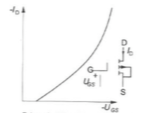
\includegraphics{./lec3/enhancement.png}
    \caption{N-type FET run in enhancement mode.}
    \ref{fig:enhancement}
\end{figure}
In depletion mode, Figure~\ref{depletion}, the FET has some resistance when $V_{GS}$ 
is at 0V. Current will the pass through DS.
\begin{figure}[H]
    \centering
    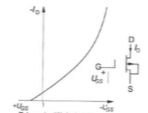
\includegraphics{./lec3/depletion.png}
    \caption{N-type FET run in depletion mode.}
    \ref{fig:depletion}
\end{figure}
